\documentclass{report}
\usepackage[T1]{fontenc} % Fontes T1
\usepackage[utf8]{inputenc} % Input UTF8
\usepackage[backend=biber, style=ieee]{biblatex} % para usar bibliografia
\usepackage{csquotes}
\usepackage[portuguese]{babel} %Usar língua portuguesa
\usepackage{blindtext} % Gerar texto automaticamente
\usepackage[printonlyused]{acronym}
\usepackage{hyperref} % para autoref
\usepackage{graphicx}
\DeclareGraphicsExtensions{.pdf,.png,.jpg, .jpeg, .gif}
\graphicspath{ {imagens/} }
\bibliography{bibliografia}


\begin{document}
%%
% Definições
%
\def\titulo{PROJETO FINAL}
\def\disciplina{Laboratórios de Informática}
\def\data{11 de junho de 2017}
\def\autores{Jorge Catarino, Francisco Martinho, Raquel Rainho, Paulo Vasconcelos}
\def\autorescontactos{(85028) jorge.catarino@ua.pt, (85088) martinho.francisco@ua.pt, (84891) raquel.a.rainho@ua.pt, (84987) paulobvasconcelos@ua.pt}
\def\versao{VERSAO}
\def\departamento{Departamento de Eletrónica, Telecomunicações e Informática}
\def\empresa{Universidade de Aveiro}
\def\logotipo{ua.pdf}
%
%%%%%% CAPA %%%%%%
%
\begin{titlepage}

\begin{center}
%
\vspace*{50mm}
%
{\Huge \titulo}\\ 
%
\vspace{10mm}
%
{\Large \empresa}\\
%
\vspace{10mm}
%
{\LARGE \autores}\\ 
%
\vspace{30mm}
%
\begin{figure}[h]
\center
\includegraphics{\logotipo}
\end{figure}
%
\vspace{30mm}
\end{center}
%
\end{titlepage}

%%  Página de Título %%
\title{%
{\Huge\textbf{\titulo}}\\
{\large {\departamento \\
        \disciplina \\
        \empresa}}
}
%
\author{%
    \autores \\
}
%
\date{\data}
%
\maketitle

\pagenumbering{roman}

%%%%%% RESUMO %%%%%%
\begin{abstract}
Que trabalhinho de merda mas pronto.

É sair daqui e ir diretamente para o UA Shitposting com um href vindo do Slack.
\end{abstract}

%%%%%% Agradecimentos %%%%%%
% Segundo glisc deveria aparecer após conclusão...
%\renewcommand{\abstractname}{Agradecimentos}
%\begin{abstract}
%Eventuais agradecimentos.
%Comentar bloco caso não existam agradecimentos a fazer.
%\end{abstract}


\tableofcontents
%\listoftables     % descomentar se necessário
%\listoffigures    % descomentar se necessário


%%%%%%%%%%%%%%%%%%%%%%%%%%%%%%%
\clearpage
\pagenumbering{arabic}

%%%%%%%%%%%%%%%%%%%%%%%%%%%%%%%%
\chapter{Introdução}
\label{chap.introducao}

Introduz o tema, apresenta a motivação e finalmente a estrutura.

Este documento está dividido em quatro capítulos.
Depois desta introdução,
no \autoref{chap.metodologia} é apresentada a metodologia seguida,
no \autoref{chap.resultados} são apresentados os resultados obtidos,
sendo estes discutidos no \autoref{chap.analise}.
Finalmente, no \autoref{chap.conclusao} são apresentadas
as conclusões do trabalho.

\chapter{Metodologia}
\label{chap.metodologia}
%introduzir ferramenta usada, descrever como foi usada
Neste capítulo vão ser expostas as várias ferramentas que a aplicação web desenvolvida irá usar, de forma a facilitar a leitura do resto do relatório.

\section{Framework}


%Módulo que apresenta um conjunto de serviços e disponibiliza uma página Web aos
%clientes, para interação com o sistema.
%Explicar!
Em termos de desenvolvimento de software, uma framework é um conjunto de código escrito previamente, que procura aumentar a eficiência do programador ao fornecer funções e funcionalidades que são comuns a várias aplicações, de forma a que o desenvolvedor não tenha que estar constantemente a programa-las, para cada aplicação.

Esta ferramenta pode ser vista como um esqueleto da aplicação, sendo que vai interligar os vários módulos necessários para o bom funcionamento desta, desde a base de dados até ao editor de imagem  
\footnote{Pode ler mais sobre estes módulos na \autoref{ssec.db} e \autoref{sec.edit}}

Neste projeto a framework usada foi Cherrypy, conforme descrito na subsecção seguinte.

\subsection{CherryPy}
CherryPy é uma framework para aplicações web desenvolvida em Python. Criada para ser o mais  pythônica, isto é, respeitando a filosofia da linguagem \footnote{Que pode ser lida com o comando "import this" no Python ou \href{https://www.python.org/dev/peps/pep-0020/}{aqui}}, esta framework permite o programador escrever uma aplicação web da mesma forma que este desenvolveria um programa para Python, o que pode resultar num código base mais compacto. 

Não só servindo como Framework, o CherryPy serve também como servidor web, com suporte a \ac{WSGI} \footnote{Pode ler mais sobre \ac{WSGI} \href{http://wsgi.readthedocs.io/en/latest/}{aqui}} 



%\subsection{Utilização de acrónimos}
%Esta é a primeira invocação do acrónimo \ac{ua}.
%E esta é a segunda: \ac{ua}.

%Outras duas referências a \ac{miect}
%e \ac{miect}.

%\subsection{Referências bibliográficas}
%Informação relativa à estrutura formal de um relatório pode ser obtida
%na página do \ac{glisc}\cite{glisc}.

\section{Página Web}

Numa aplicação web destinada a uso comercial, o front-end tem uma importância extrema. Sendo o único módulo que o usuário comum normalmente interage, é crucial que este seja intuitivo e atrativo, pois, mesmo que o back-end esteja completamente funcional, uma aplicação difícil de usar e olhar, também dificilmente atraíra utilizadores. É também relevante garantir compatibilidade para o maior número de Browsers e aparelhos possível. 

Para tal, foi utilizado a framework Ratchet.

\subsection{Ratchet}

Ratchet é uma framework open-source para desenvolvimento de front-end mobile, com HTML, CSS e JavaScript. Esta ferramenta permite criar páginas Web, que podem posteriormente ser adaptadas para vários aparelhos diferentes, desde telemóveis a tablets. Foi desenvolvida por três ex-programadores do Twitter, enquanto desenvolviam a aplicação mobile da rede social. Continua a ser desenvolvida atualmente por um dos criadores e pela comunidade. 

Na figura pode-se ver um exemplo genérico de uma aplicação que use esta framework, a correr num IPhone.

\begin{figure}[!htb]
\label{fig.ratex}
\centering
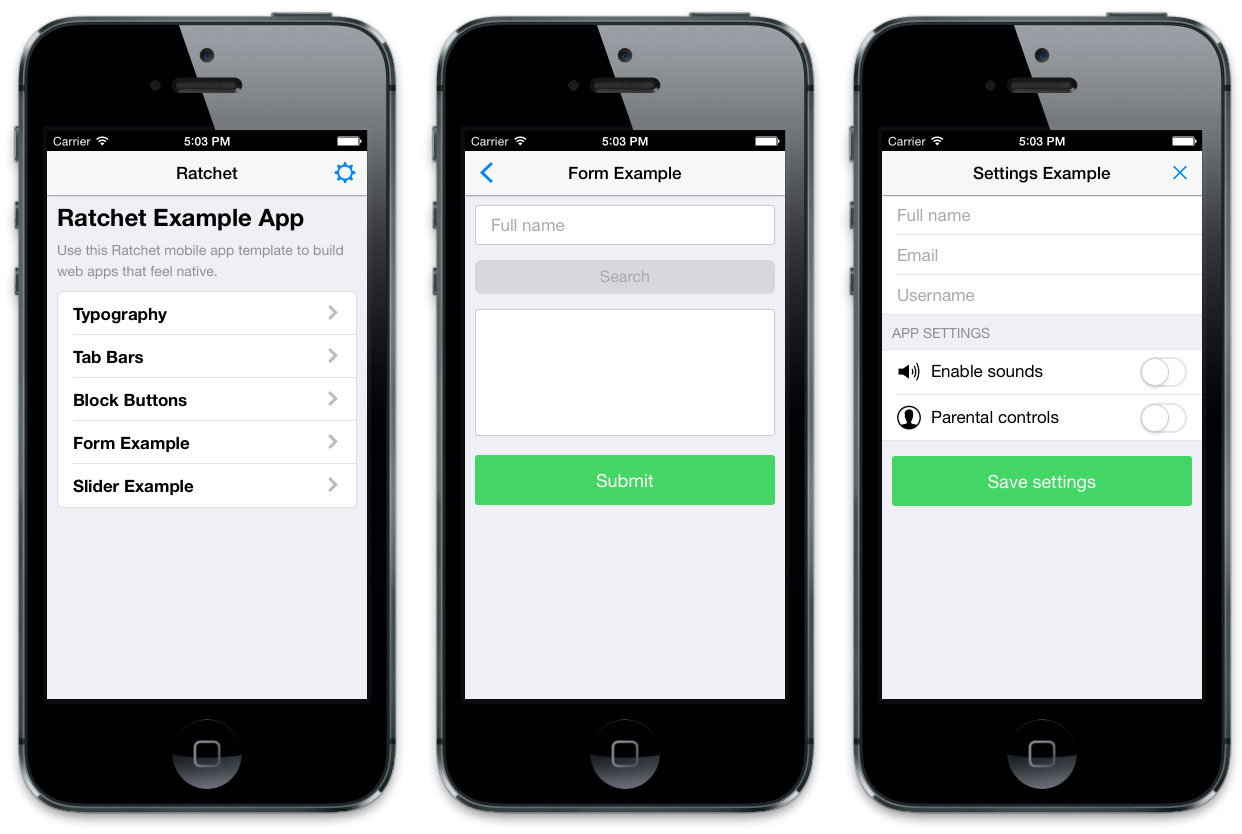
\includegraphics[scale=0.19]{ratchet-example}
\caption[Exemplo de Ratchet]{Exemplo de uma Aplicação Ratchet}
\end{figure}

\section{Persistência}
\subsection{Base de Dados}
\label{ssec.db}
Uma base de dados é uma ferramenta que tem a capacidade de armazenar e organizar grande quantidade de informação, independentemente do que esta seja. 

Com o uso de um \ac{DBMS} , podemos aceder aos dados nela guardados, podendo pesquisar por certos elementos, adicionar novos dados, atualizar as informações mais antigos e apagar o que já não for necessário, entre outras funções.

Ao longo dos anos, foram desenvolvidos vários modelos de base de dados, começando com o modelo de navegação, popularizado nos anos 60, até as mais recentes bases de dados em XML.

O modelo que irá ser usado neste projeto é o modelo Relacional.

\subsubsection{Base de Dados Relacional}
%falar do modelo relacional
%Edgar Frank COdd
%como é que são guardados os dados e como eles se relacionam
%falar de sqlite3
%meter imagens
Uma base de dados relacional é uma coleção de vários itens de informação, organizada por tabelas, estas podendo ser acedidas conforme necessário, sem ter de ser reorganizadas. Este modelo foi inventado por E.F.Codd, em 1970, na IBM. 

Este modelo destacasse pelo facto de ser possível identificar cada fila de uma tabela, com uma chave única de qualquer tipo, que se dá o nome de chave primária.

É também possível relacionar várias tabelas, através de chaves estrangeiras, isto é, pondo a chave primária de uma tabela noutra.
\begin{figure}[!htb]
\label{fig.dbrel}
\centering
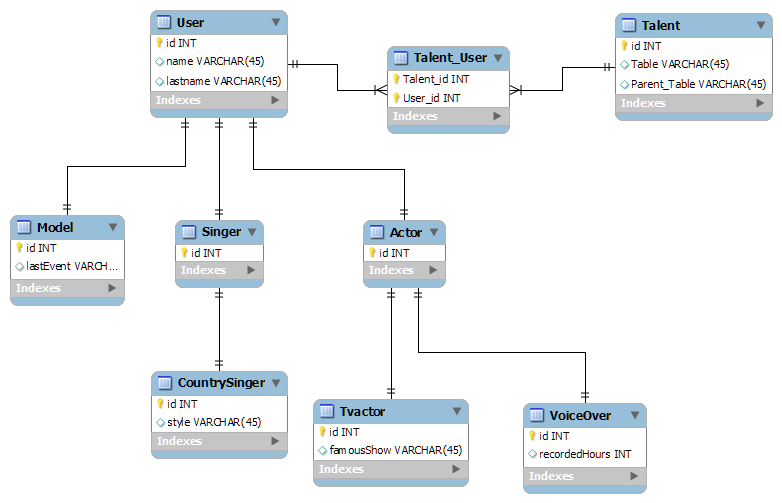
\includegraphics[scale=0.2]{DBRel}
\caption[Ilustração de uma base de dados relacional]{Na figura encontra-se o desenho de uma base de dados relacional}
\end{figure}

Neste projeto, para aceder a base de dados, vai ser usado SQLite, uma DBMS que não necessita de configuração e que não necessita de um servidor para funcionar. Por estas e outras razões, a popularidade desta DBMS tem crescido ao longo dos anos, sendo usada em aplicações como o Facebook e o Firefox.

Este gestor tem a linguagem de programação SQL implementada nele, pelo que os acessos a base de dados vão ser feitos via queries usando esta linguagem.
\section{Edição de Imagem}
\label{sec.edit}

Edição de imagem é o processo de alterar uma fotografia  de modo a atingir certos objetivos, seja cortar um certo elemento intrusivo, realçar cores ou inserir novos elementos. Este programa deverá ser capaz de aplicar alguns efeitos a imagens e de criar memes, sendo este processo exposto nas subsecções seguintes e demonstrado no \autoref{chap.resultados} 
\subsection{Módulo de Efeitos}



\subsection{Módulo de memes}

Meme é um termo amplo. A palavra, cunhada por Richard Dawkins no livro \textbf{\textit{"O Gene Egoísta"}}  publicado em 1976, onde o autor tentava explicar a maneira como a cultura se espalhava, era usada para descrever qualquer ideia, comportamento ou estilo que passava de pessoa a pessoa dentro de uma determinada cultura. 


Na cultura da internet, memes podem vir em vários formatos, desde pequenos textos, músicas, vídeos e imagens, normalmente com fins humorísticos. 


A aplicação desenvolvida deverá ser capaz de criar um formato de internet meme famoso, o image macro, que consiste de uma imagem com texto sobreposto, normalmente na fonte Impact.

\begin{figure}[!htb]
\label{fig.meme}
\centering

\includegraphics[scale=0.6]{meme}
\caption[Exemplo de Image Macro]{Exemplo de um image macro que pode ser encontrado na web}
\end{figure}

A semelhança do outros efeitos, para editar a imagem vai ser usada a \ac{PIL}

\chapter{Resultados}
\label{chap.resultados}
Descreve os resultados obtidos.

\chapter{Análise}
\label{chap.analise}
Analisa os resultados.

\chapter{Conclusões}
\label{chap.conclusao}
Apresenta conclusões.

\chapter*{Contribuições dos autores}
(RR) - Raquel Rainho
(JC) - Jorge Catarino
(PV) - Paulo Vasconcelos
(FM) - Francisco Martinho

%%%%%%%%%%%%%%%%%%%%%%%%%%%%%%%%%
\chapter*{Acrónimos}
\begin{acronym}
\acro{ua}[UA]{Universidade de Aveiro}
\acro{miect}[MIECT]{Mestrado Integrado em Engenharia de Computadores e Telemática}
\acro{lei}[LEI]{Licenciatura em Engenharia Informática}
\acro{glisc}[GLISC]{Grey Literature International Steering Committee}
\acro{DBMS}[DBMS]{Database Management System}
\acro{PIL}[PIL]{Python Imaging Library}
\acro{WSGI}[WSGI]{Web Server Gateway Interface}
\end{acronym}


%%%%%%%%%%%%%%%%%%%%%%%%%%%%%%%%%
\printbibliography

\end{document}
